\chapter{Results}
\label{cha:result}
\lettrine[lines=4, loversize=-0.1, lraise=0.1]{D}{uring the project} experiments were conducted to evaluate state of practice speech recognition and the efficiency and scalability as well as the usefulness of the developed system. The following sections will present the results of these experiments.

\section{Speech Recognition}
This section will present the findings from the experiments on speech recognition, see Section~\ref{sec:reqmatchexp} and Section~\ref{sec:speechrecacc}. The data from the experiments can be found in Appendix~\ref{app:reqmatchexpres} and Table~\ref{tab:recaccexp}.

\subsection{Recognition Accuracy}
\label{subsec:recaccresult}
The results from the Recognition Accuracy Experiment~(see~\ref{sec:speechrecacc}) in Table~\ref{tab:recaccexp} shows that free text speech input is not good enough to provide accurate descriptions as of now. As many as 64\% are not comprehensible, and 10\% can introduce errors if interpreted as written. The number of samples is 98 rather than the stated 100 in the Method chapter (see Chapter~\ref{chap:meth}), this is because the experiment equipment failed to record two of the inputs from two different subjects.
\begin{table}[h]
\centering
\caption{Number of descriptions in each severity ranking.}
    \begin{tabular}{ l  p{2cm}  p{7.5cm} }
        \hline
        Severity & Frequency (n=98) & Explanation \\
        \hline
        0 & 8 & No error\\
        1 & 17 &  Minor error, still comprehensible\\
        2 & 63 &  Error, hard/impossible to comprehend\\
        3 & 10 & Severe Error, meaning of text has changed, but has a viable meaning in the context\\
        \end{tabular}
\label{tab:recaccexp}
\end{table}

\FloatBarrier

\subsection{Requirement Matching}
\label{sub:reqmatch}
The requirement matching experiment showed that a string edit distance algorithm such as Levenshtein's edit distance can give satisfiable results for matching natural language to name conventions used in an SRS. When the speech recognizers interpreted input of the subjects spoken title of requirements was run through the Levenshtein edit distance algorithm and used towards an SRS of 4544 requirements, 93\% ended up in the rank of one to five. Figure \ref{fig:freqperrank} shows a graph for the percentage of requirements that was ranked among the N top requirements. From the graph we can see that for 73\% of the requirements the target requirement was top ranked and in 93\% of the cases the target rank was among the top five among the 4544 requirements in this SRS.
The mean rank was $6.96$ but this is dominated by a few requirements where the speech recognizer gave output very far from the target requirement; the median rank was 1.


\begin{figure}[h]
\centering
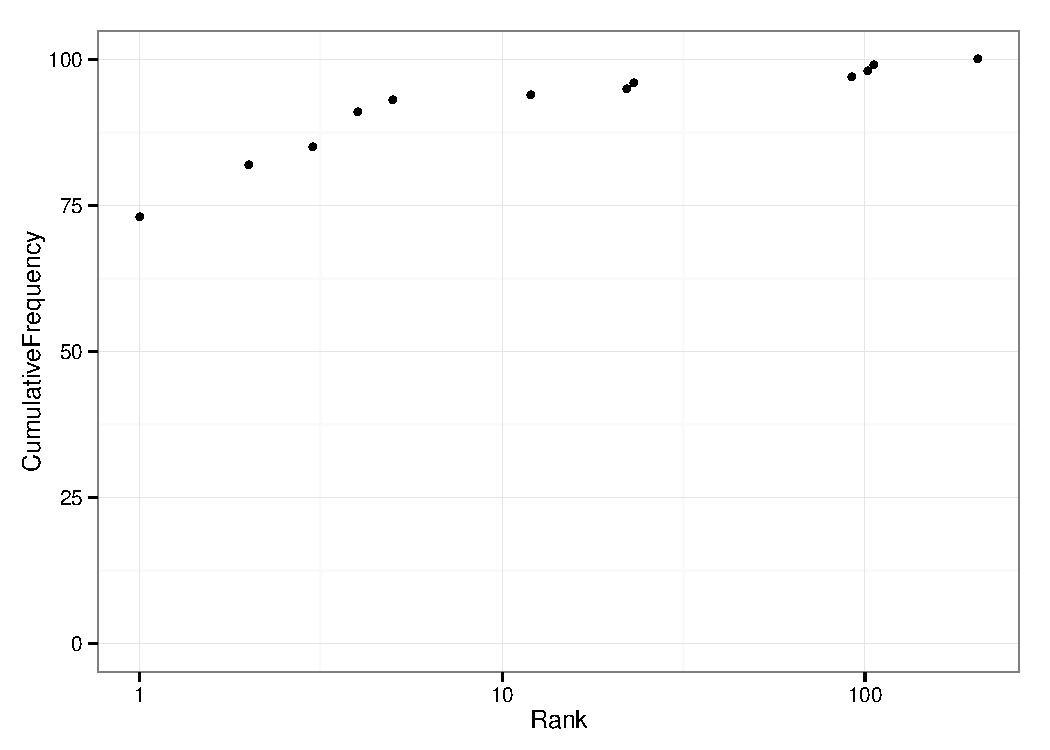
\includegraphics[width = 350pt, keepaspectratio = true]{fig/freqperrank}
\caption{Graph showing the cumulative frequency and the edit distance rank}
\label{fig:freqperrank}
\end{figure}

The speech recognizer delivered 15 perfect matches, and of these 12 where at the first position of the returned results from the speech recognizer. In two of the cases the perfect match was at the speech recognizer's second result, and in one of the cases the perfect match was at the fifth result. In all of the cases, the input to the Levenshtein edit distance algorithm (i.e.\ the first result returned from the speech recognizer) had the Levenshtein rank 1. The ranges of the inputs that resulted in perfect matches were between 15 to 43 characters, this is most likely because longer strings are more vulnerable to error since any word can be misinterpreted, shorter requirement titles seemed to contain more abbreviations and symbols such as "->" or parentheses/brackets, presumably a consequence of that the recognizer's expected input is words of natural language. None of the given input returned a false perfect match.


\begin{figure}[h]
\centering
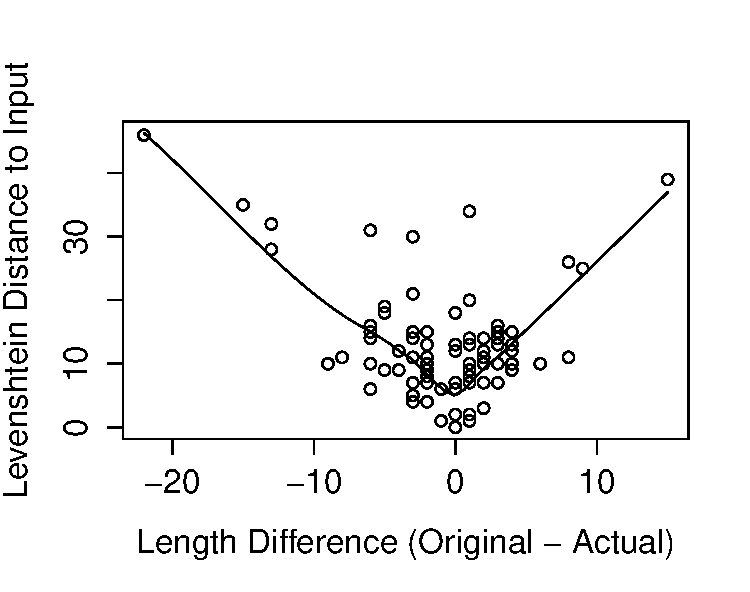
\includegraphics[width = 250pt, keepaspectratio = true]{fig/levdif}
\caption{The Levenshtein distance and its correlation with the difference in input length, the line shows a locally fitted regression.}
\label{fig:levdif}
\end{figure}

\FloatBarrier

The correlation between Levenshtein distance to the sought requirement title and the difference in length between input and what the speech recognition interpreted can be seen in Figure~\ref{fig:levdif}. This figure shows that the Levenshtein distance gives better results for strings with similar length. Since the input and interpreted string length often is quite close, this gives good results. This also gives a hint that it's better for the user to try to pronounce the whole title, even hard to pronounce symbols and abbreviations to make the matching better.

A table with the data gathered from the experiment is shown in Appendix~\ref{app:reqmatchexpres}

\section{Large Scale Requirements Engineering}
\label{eval:lsre}
Approximate times for the different look-ups are described in Table~\ref{tab:timetype} and~\ref{tabl:explsre}. The times shown are from the start of the look-up on the SpeechServer, until the SpeechServer has returned the items and is ready to send to the client. This shows that even for large scale requirements engineering these kinds of operations are feasible. The times in Table~\ref{tab:timetype} shows that the number of projects (and contexts within a project) are so low that the times are irrelevant. The time to look up requirements takes a bit longer as can be seen in Table~\ref{tabl:explsre}. SpeechServer and SystemWeaver is running on a laptop with an dual core Intel i5-350 processor with hyper-threading and 4GB RAM.

The times to look up items is sometimes unpredictable since SystemWeaver as well as SpeechServer does caching internally, this depends on what has been searched before and other factors, such as other users and how much can be cached. These results however are close to what can be expected. How the user perceives the interaction is discussed in Section~\ref{sec:ux}.

\begin{table}[h]
\centering
\caption{Approximate times to look up projects and contexts, mean of 10 runs.}
\centering
    \begin{tabular}{l l l}
        \hline
        Type & Quantity & Time in ms \\
        \hline
        Projects & 89 & 2 \\
        Contexts & 3 & 1 \\
        \end{tabular}
\label{tab:timetype}
\end{table}

\begin{table}[h]
\centering
\caption{Times to look up item requirements, mean of 31 runs.}
\centering
    \begin{tabular}{l  l}
        \hline
        Requirements & Time in ms \\
        \hline
        4544 & 1450 \\
        959 & 39 \\
        210 & 209 \\
        2548 & 797
        \end{tabular}
\label{tabl:explsre}
\end{table}

\begin{figure}[h]
\centering
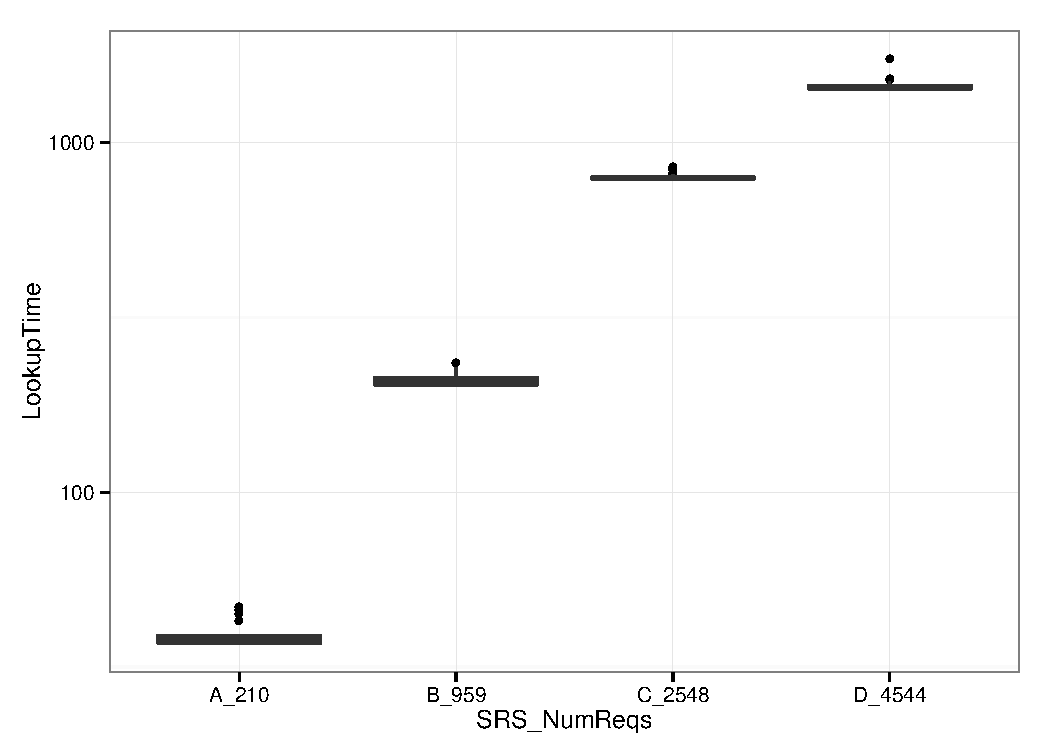
\includegraphics[width = 350pt, keepaspectratio = true]{fig/boxplots}
\caption{The boxplots show the distribution of the 31 runs for the different sizes.}
\label{fig:boxplots}
\end{figure}

\FloatBarrier

\section{Product Evaluation}
\label{sec:prodeval}
The product was evaluated through a user-test and a following interview. What lied in focus during the interview was the annotations that were created in themselves, but also the user's experience of the application. The results from this interview will be divided into two parts, the annotations and the usefulness of those, and the overall experience of the application.

\subsection{Annotations on Softer Artefacts}
All of the interviewed subjects used TODO-lists in the format of analog or digital notes to their ongoing projects. However, what they found to be a huge profit with the annotations on the requirements was that there were a direct connection between the TODO-entity (the annotation) and the actual requirement. 

A factor that was considered as very important for all of the interviewees were the content of the annotations. They found it very important that the naming of the annotations fitted the way they worked with maintenance of projects, and that there needed to be a clear definition and distinction between each and one of the annotations. The interviewees expressed that the annotations without any more descriptive information (a file or a description field) were better for peer-reviewing purposes (i.e.\ letting users go through the SRS and go through the annotations in a group format), where as an annotation that contained descriptive information were better for actual modifications and improvements on the requirement. 

\subsection{User Experience}
\label{sec:ux}

The key notes that the subjects expressed as very positive was the accuracy and the response time of the application. 

Many subjects expressed the usefulness of the mobility in the application. To be able to query an SRS with several thousand of requirements anywhere, from the car or the bar, was considered a huge advantage. The solution was also considered very lightweight, and the flow combined with the low amount of time to create an issue were expressed as an easy solution to directly ventilate their thoughts towards the SRS, instead of a tidy operation when they would otherwise have to make several operations to navigate and interact with SystemWeaver.

Some felt uncomfortable using speech as the main input for the application. Moreover, requirement titles that contained special characters (e.g.\ "\#", "->", "=") or abbreviations were found hard translate to spoken words. Another problem that was pointed out was the sound that was produced during the operation, and several of the subjects stated that it might not be so good to use it in shared environments. 


